\documentclass{beamer}
\usetheme{Malmoe}
%\usepackage{beamerthemesplit} %// Activate for custom appearance
%\setbeamertemplate{footline}[page number]{}
\usepackage{graphicx,subfig,float}


\title{Some Prediction of White Wine Grading}
\author[Chung, K.I. and Xiao, B.J.]{Chung, K.I. and Xiao, B.J.\\{\small Supervised by: Prof. Lo, M.N. }}
\date{January 13, 2017}

\begin{document}

\frame{\titlepage}
%%%% outline %%%%
\section[Outline]{}
\frame{\tableofcontents}

%%%%  introduction %%%%
\section{Introduction}
%% Overview %%
\subsection{Overview of the Data}
\frame{
\frametitle{Overview of the Data}
	\begin{columns}
		\begin{column}{0.5\textwidth}
			\begin{itemize}
				\item {From the UC Irvine Machine Learning Repository Website}
				\item{4898 Observations and 12 variables}
				\item{4408 training data and 490 test data}
			\end{itemize}

		\end{column}
  		\begin{column}{0.5\textwidth}
			\begin{figure}
    				\begin{center}
        					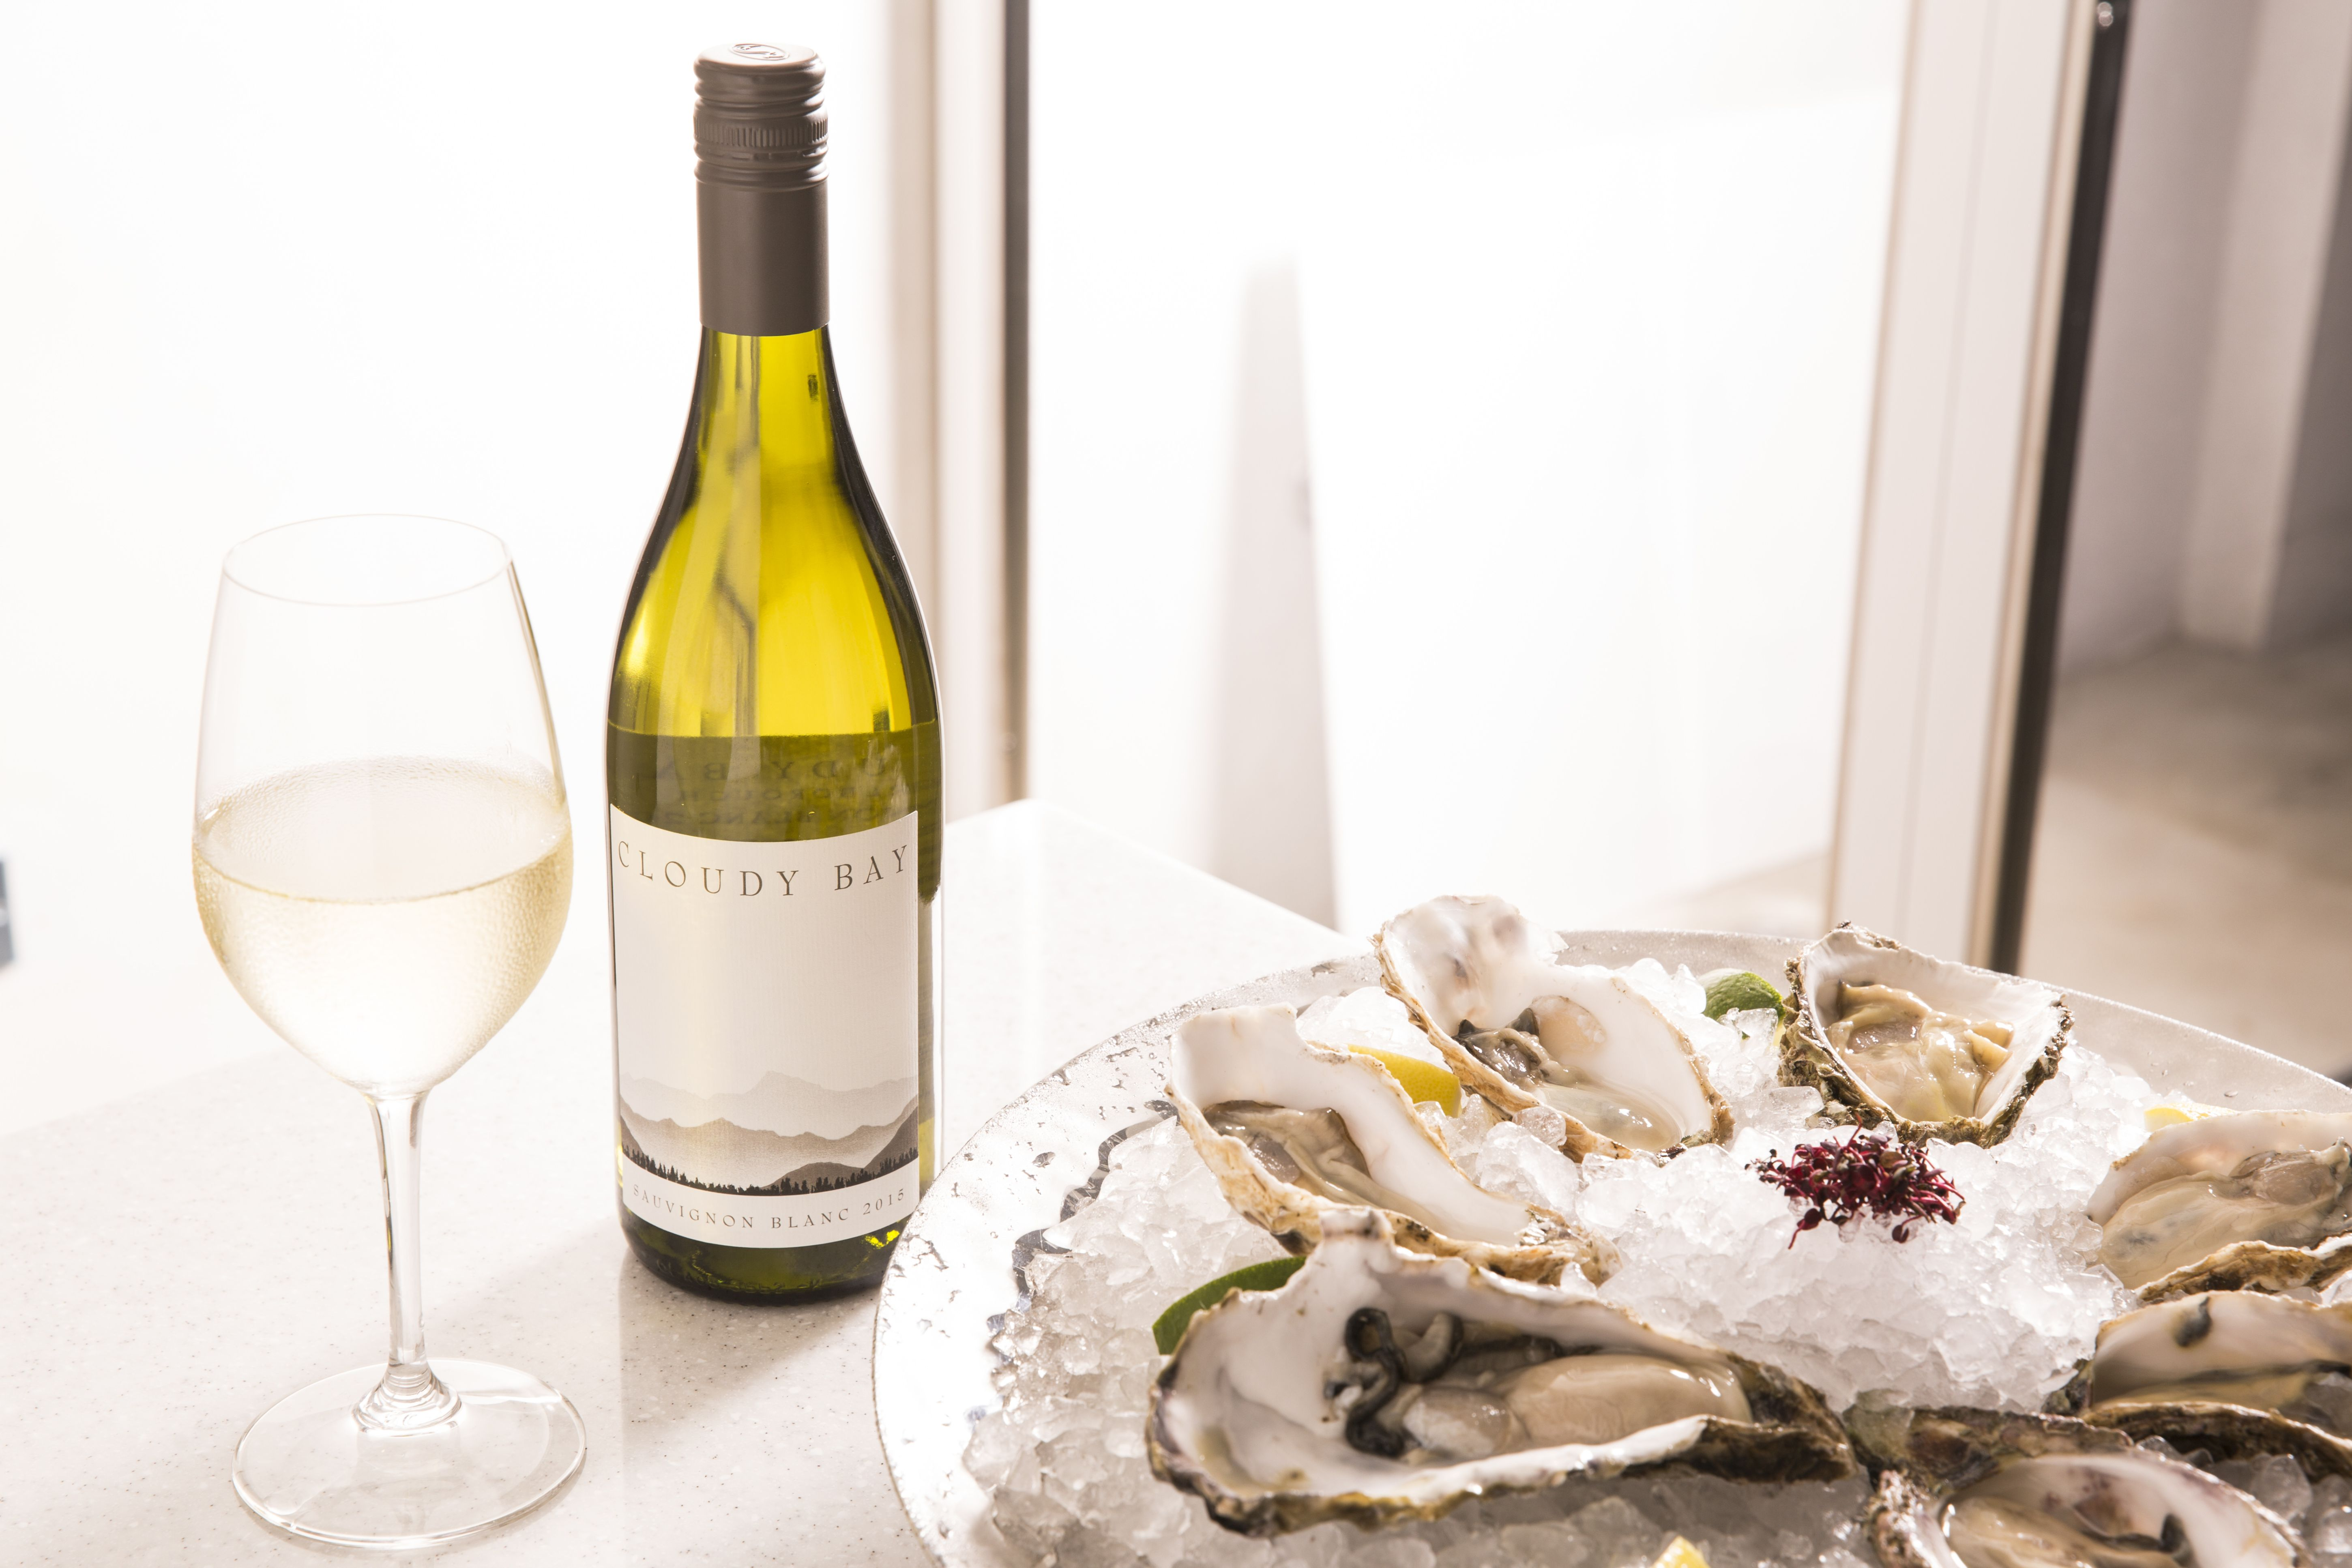
\includegraphics[width=160pt]{figure/Wine_1.png}
        				\end{center}
			\end{figure}
		\end{column}
	\end{columns}
}

\frame{
\frametitle{Response}
\qquad The quality of the the wine is  graded from 3 to 9.
\begin{table}[htp]
		\begin{center}
			\begin{tabular}{c|ccccccc}
	                      	Grade		&	3	&	4	&	5	&	6	&	7	&	8	&	9\\ \hline
				Frequency	&	20	&	163	&	1457	&	2198	&	880	&	175	&	5
			\end{tabular}
		\end{center}
	\label{default}
\end{table}
}	

\frame{
\frametitle{Predictors}
	\begin{columns}
		\begin{column}{0.5\textwidth}
			\begin{itemize}
				\item {Fixed acidity ($g/l$)}
				\item{Volatile Acidity ($g/l$)}
				\item{Citric Acid ($g/l$)}
				\item{Residual Sugar ($g/l$)}
				\item{Chlorides ($g/l$)}
			\end{itemize}
		\end{column}
 		\begin{column}{0.5\textwidth}
			\begin{itemize}
				\item {Free Sulfur Dioxide ($mg/l$)}
				\item{Total Sulfur Dioxide ($mg/l$)}
				\item{Density ($g/ml$)}
				\item{pH}
				\item{Sulphate (g/l)}
				\item{Alcohol (\%)}
			\end{itemize}
		\end{column}
	\end{columns}
}
\frame{
\frametitle{Target}
\begin{itemize}
		\item{Find the relation between the variables}
		\item{Predict the quality of the wine}
		\item{Reduce the error rate}
\end{itemize}
}

%%%% Correlation and PCA %%%%
% \section{Relation between the Variables}
%% Correlation %%
\subsection{Correlation}
\frame{
			\begin{table}[htp]
				\caption{Coefficient Matrix}
				\resizebox{\textwidth}{!}{
					\begin{center}
						\begin{tabular}{rrrrrrrrrrrr}
1 & -0.02 & 0.28 & 0.09 & 0.02 & -0.05 & 0.09 & 0.26 & -0.42 & -0.02 & -0.11 & -0.11 \\
-0.02 & 1 & -0.14 & 0.06 & 0.07 & -0.1 & 0.09 & 0.03 & -0.04 & -0.03 & 0.07 & -0.19 \\
0.28 & -0.14 & 1 & 0.09 & 0.11 & 0.09 & 0.11 & 0.15 & -0.16 & 0.07 & -0.07 & -0.01 \\ 
 0.09 & 0.06 & 0.09 & 1 & 0.09 & 0.29 & 0.40 & 0.84 & -0.19 & -0.03 & -0.45 & -0.10 \\
 0.02 & 0.07 & 0.11 & 0.09 & 1 & 0.11 & 0.2 & 0.26 & -0.09 & 0.02 & -0.36 & -0.21 \\
-0.05 & -0.10 & 0.09 & 0.29 & 0.11 & 1 & 0.61 & 0.29 & 0.00 & 0.06 & -0.25 & 0.01 \\
0.09 & 0.09 & 0.11 & 0.40 & 0.20 & 0.61 & 1 & 0.53 & 0.00 & 0.14 & -0.45 & -0.17 \\
0.26 & 0.03 & 0.15 & 0.84 & 0.26 & 0.29 & 0.53 & 1 & -0.09 & 0.08 & -0.78 & -0.30 \\
-0.42 & -0.04 & -0.16 & -0.19 & -0.09 & 0.00 & 0.00 & -0.09 & 1 & 0.16 & 0.12 & 0.10 \\
-0.02 & -0.03 & 0.07 & -0.03 & 0.02 & 0.06 & 0.14 & 0.08 & 0.16 & 1 & -0.03 & 0.05 \\
 -0.11 & 0.07 & -0.07 & -0.45 & -0.36 & -0.25 & -0.45 & -0.78 & 0.12 & -0.03 & 1 & 0.43 \\
 -0.11 & -0.19 & -0.01 & -0.10 & -0.21 & 0.01 & -0.17 & -0.30 & 0.10 & 0.05 & 0.43 & 1
						\end{tabular}
					\end{center}
					}
				\label{default}
			\end{table}
}
%fixed.acidity & -0.02 & 0.28 & 0.09 & 0.02 & -0.05 & 0.09 & 0.26 & -0.42 & -0.02 & -0.11 & -0.11 \\
%-0.02 & volatile.acidity & -0.14 & 0.06 & 0.07 & -0.1 & 0.09 & 0.03 & -0.04 & -0.03 & 0.07 & -0.19 \\
%0.28 & -0.14 & citric.acid & 0.09 & 0.11 & 0.09 & 0.11 & 0.15 & -0.16 & 0.07 & -0.07 & -0.01 \\ 
% 0.09 & 0.06 & 0.09 & residual.sugar & 0.09 & 0.29 & 0.40 & 0.84 & -0.19 & -0.03 & -0.45 & -0.10 \\
% 0.02 & 0.07 & 0.11 & 0.09 & chlorides & 0.11 & 0.2 & 0.26 & -0.09 & 0.02 & -0.36 & -0.21 \\
%-0.05 & -0.10 & 0.09 & 0.29 & 0.11 & free.sulfur.dioxide & 0.61 & 0.29 & 0.00 & 0.06 & -0.25 & 0.01 \\
%0.09 & 0.09 & 0.11 & 0.40 & 0.20 & 0.61 & total.sulfur.dioxide & 0.53 & 0.00 & 0.14 & -0.45 & -0.17 \\
%0.26 & 0.03 & 0.15 & 0.84 & 0.26 & 0.29 & 0.53 & density & -0.09 & 0.08 & -0.78 & -0.30 \\
%-0.42 & -0.04 & -0.16 & -0.19 & -0.09 & 0.00 & 0.00 & -0.09 & pH & 0.16 & 0.12 & 0.10 \\
%-0.02 & -0.03 & 0.07 & -0.03 & 0.02 & 0.06 & 0.14 & 0.08 & 0.16 & sulphates & -0.03 & 0.05 \\
 %-0.11 & 0.07 & -0.07 & -0.45 & -0.36 & -0.25 & -0.45 & -0.78 & 0.12 & -0.03 & alcohol & 0.43 \\
 %-0.11 & -0.19 & -0.01 & -0.10 & -0.21 & 0.01 & -0.17 & -0.30 & 0.10 & 0.05 & 0.43 & quality
\frame{
			\begin{figure}
    				\begin{center}
        					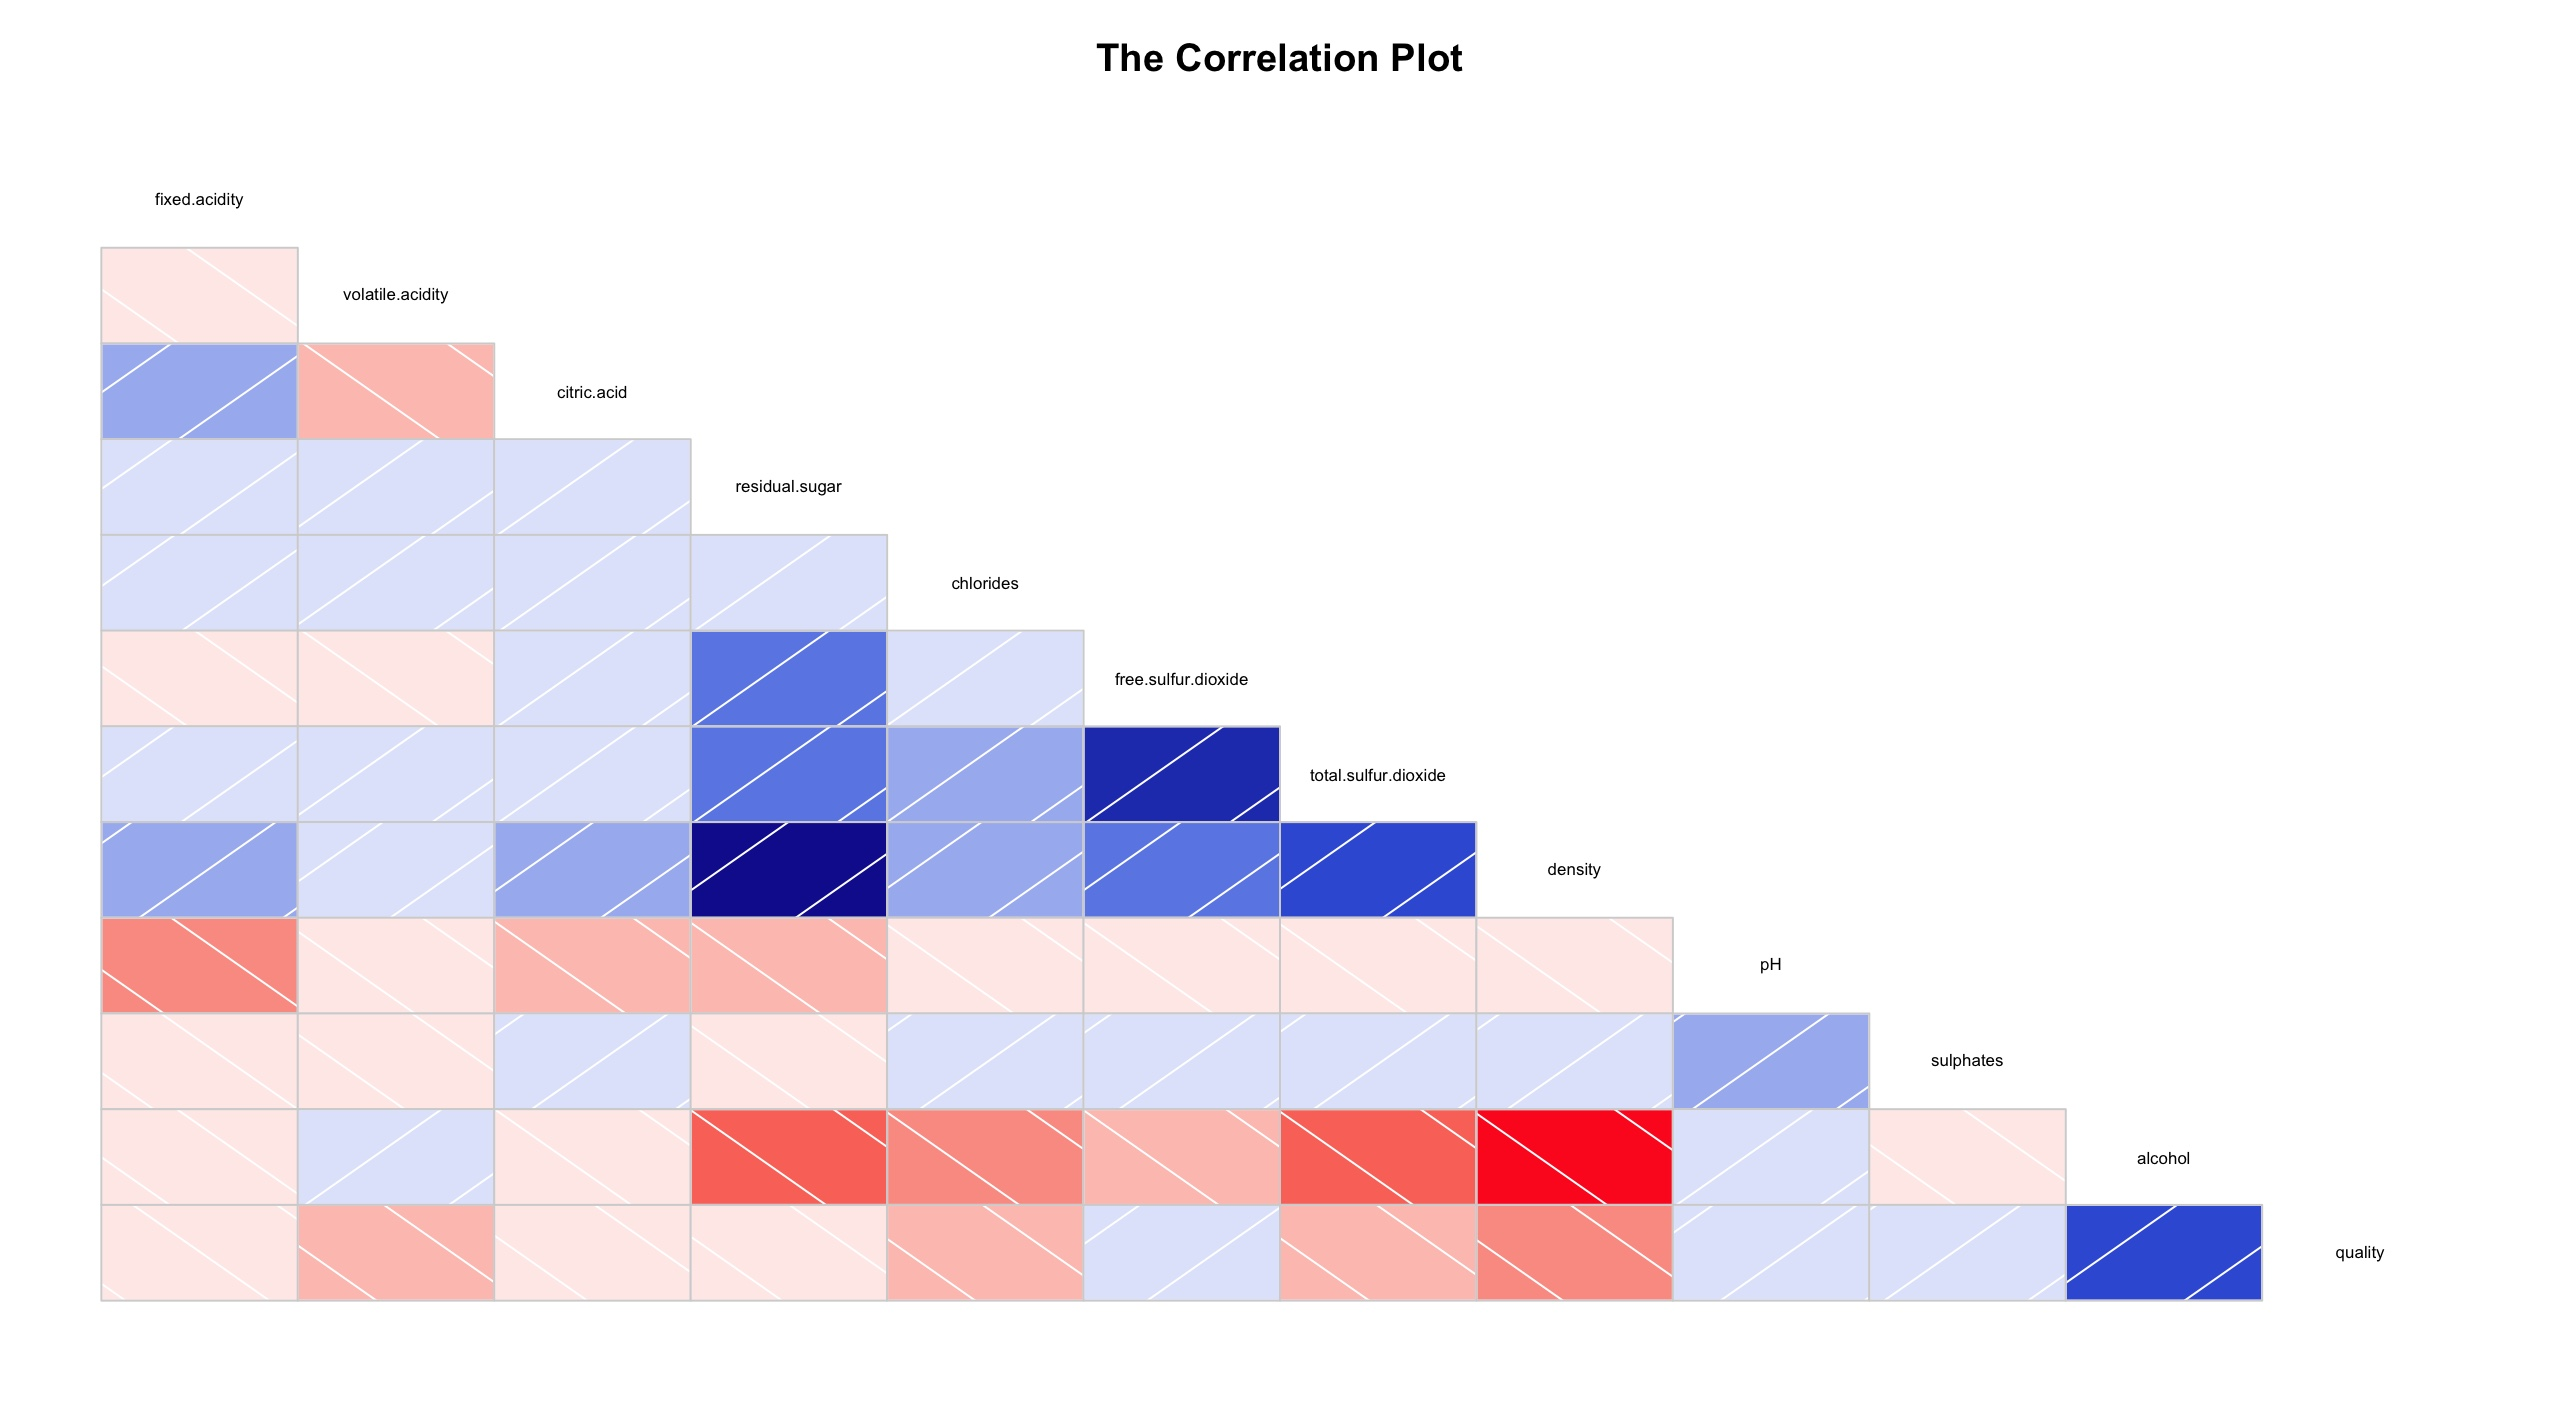
\includegraphics[width=330pt]{figure/Corr.png}
        				\end{center}
			\end{figure}
}


\subsection{PCA}
\frame{
			\begin{table}[htp]
				\caption{PCA output}
				\resizebox{\textwidth}{!}{
					\begin{center}
						\begin{tabular}{crrrrrrrr}
                      	& PC1 &  PC2  & PC3  & PC4  & PC5  & PC6  & h2  &  u2 \\
fixed.acidity       &  0.28& \alert{-0.74} & 0.13  &0.02&  0.25 &-0.10 &0.71& 0.287 \\
volatile.acidity    &  0.01  &0.06 &\alert{-0.65}  &0.28  &0.63 & 0.12 &0.92& 0.077 \\
citric.acid           &0.26& -0.43 & \alert{0.56} & 0.15 & 0.05 & 0.13& 0.61 &0.393 \\
residual.sugar    &    \alert{0.77} & 0.01 &-0.24& -0.28  &0.01& -0.28& 0.80 &0.200 \\
chlorides             &0.38 &-0.01& -0.11 & \alert{0.72} &-0.32 & 0.38& 0.92& 0.076 \\
free.sulfur.dioxide  & \alert{0.54}  &0.36 & 0.31& -0.31 & 0.17 & 0.48& 0.87 &0.126 \\
total.sulfur.dioxide & \alert{0.73} & 0.31 & 0.14 &-0.06 & 0.29&  0.27 &0.80& 0.195 \\
density              & \alert{0.92}  &0.01 &-0.14 &-0.02& -0.08& -0.32& 0.97 &0.028 \\
pH                   &-0.23 & \alert{0.73} & 0.14 & 0.10 &-0.12 &-0.19 &0.66 &0.336 \\
sulphates          &   0.08  &0.28 & 0.48 & 0.45 & 0.40 &-0.47& 0.89 &0.114 \\
alcohol             & \alert{-0.78}& -0.04 & 0.12& -0.14 & 0.33 & 0.13& 0.78& 0.219 \\ \hline
SS loadings          & 3.22 &1.58& 1.22 &1.02& 0.97 &0.94 & & \\
Proportion Var       & 0.29& 0.14 &0.11& 0.09 &0.09 &0.09& & \\
Cumulative Var       & 0.29& 0.44 &0.55 &0.64 &0.73 &0.81& & \\
Proportion Explained  &0.36 &0.18& 0.14& 0.11& 0.11 &0.10& & \\
Cumulative Proportion &0.36 &0.54 &0.67 &0.79 &0.90 &1.00& & 
						\end{tabular}
					\end{center}
					}
				\label{default}
			\end{table}
}

%%%% LM %%%%
\section{Multiple Linear Regressions}
%% Procedure %%
\subsection{Procedure}

\frame{
\frametitle{Procedure}
	\begin{itemize}
		\item[1] {Fit a multiple linear regression with training data}
		\item[2] {Predict the response of the test data}
		\item[3] {Calculate the test MSE}
		\item[4] {Round off the predictions to integers range from 3 to 9}
		\item[5] {Calculate the test error rate}
	\end{itemize}
}

%% Regular Way %%
\subsection{Regular Model Selection Method}
\frame{
\frametitle{Full Model}
			\begin{table}[htp]
				\caption{Coefficients of the Full Model}
				\resizebox{\textwidth}{!}{
					\begin{center}
						\begin{tabular}{rrrr}
         (Intercept)     &   fixed.acidity  &   volatile.acidity     &     citric.acid \\
            137.5716         &      0.0569       &       -1.8633         &      0.0315 \\ \hline
      residual.sugar       &     chlorides  &free.sulfur.dioxide &total.sulfur.dioxide \\
              0.0771     &         -0.3096         &      0.0039      &        -0.0003 \\ \hline
             density         &          pH         &   sulphates      &        alcohol \\
           -137.4853       &        0.6397     &          0.5982     &          0.2074   
						\end{tabular}
					\end{center}
					}
				\label{default}
			\end{table}
}

\frame{
\frametitle{Collinearity Elimination}
\qquad The following table shows that the predictors residual.sugar, density and alcohol as relatively high collinearity.
			\begin{table}[htp]
				\caption{VIF of the Full Model}
				\resizebox{\textwidth}{!}{
					\begin{center}
						\begin{tabular}{rrrr}
       fixed.acidity   &  volatile.acidity     &     citric.acid     &  residual.sugar \\
              2.6444     &          1.1449         &      1.1562        &       \alert{12.5508} \\ \hline
           chlorides & free.sulfur.dioxide& total.sulfur.dioxide       &       density \\
              1.2390       &        1.7795         &      2.2262      &        \alert{27.8343} \\ \hline
                  pH        &    sulphates       &       alcohol & \\ 
              2.1600        &       1.1422        &        \alert{7.5554} &
						\end{tabular}
					\end{center}
					}
				\label{default}
			\end{table}
}

\frame{
\qquad To eliminate the the effect of the collinearity, we will perform the "leave-one-in" model selection which provide us the least AIC model with one of three collinear predictors.
			\begin{table}[htp]
				\caption{AIC of the Three Candidates}
				
					\begin{center}
						\begin{tabular}{ccc}
						residual.sugar      &  density    &    alcohol \\
      						10941.64     &  10722.53    &   \alert{10195.19} 
						\end{tabular}
					\end{center}
					
				\label{default}
			\end{table}
}

\frame{
\frametitle{Insignificant Predictor Detection}
			\begin{table}[htp]
				\caption{P-value of the Model without Collinearity}
				\resizebox{\textwidth}{!}{
					\begin{center}
						\begin{tabular}{cccc}

         (Intercept)     &   fixed.acidity  &   volatile.acidity     &     citric.acid \\
                0.00        &         0.00          &       0.00         &        \alert{0.70} \\ \hline
           chlorides  &free.sulfur.dioxide &total.sulfur.dioxide       &            pH \\ 
                0.00          &       0.00         &        \alert{0.47}         &        \alert{0.75} \\ \hline
           sulphates        &      alcohol  & &	\\ 
                0.00          &       0.00     & &	
						\end{tabular}
					\end{center}
					}
				\label{default}
			\end{table}
}

\frame{
\frametitle{The Final Model}
			\begin{table}[htp]
				\caption{Coefficients of the Final Model}
				\resizebox{\textwidth}{!}{
					\begin{center}
						\begin{tabular}{cccc}
         (Intercept)    	&    	fixed.acidity   	&  	volatile.acidity  	&    citric.acid 	\\
              3.1023       	&      	-0.0588           	&   	-1.8977        	&       0.0221 	\\ \hline
 free.sulfur.dioxide 	&total.sulfur.dioxide  	&  	alcohol 		&	  		\\
              0.0055        	&  	-0.0001           	&    	0.3345   		& 			\\
						\end{tabular}
					\end{center}
					}
				\label{default}
			\end{table}
}

\frame{
\frametitle{The Test MSE and the Test Error Rate}
			\begin{table}[htp]
				\caption{Error Table}
					\begin{center}
						\begin{tabular}{cccc}
& Full & Without Collinearity & Final \\ \hline
MSE& 0.705 &0.724& 0.727 \\
Err. Rate& 0.465 &0.469 &0.473
						\end{tabular}
					\end{center}
				\label{default}
			\end{table}

	\begin{columns}
		\begin{column}{0.33\textwidth}
			\begin{table}[htp]
				\resizebox{\textwidth}{!}{
					\begin{center}
						\begin{tabular}{c|ccccccc}
   & & & & tru & & & \\
prd  & 3  & 4 &  5 &  6 &  7 &  8 &  9\\  \hline
  3& 0& 0& 0& 0& 0& 0& 0 \\
  4 & 0 &1 &  2  & 0  & 0  & 0 &  0   \\
  5 &  0 &  8 & 61 & 27 &  0 &  0 &  0\\
  6 &  0  & 6 & 79 &184 & 69  & 9  & 1\\
  7  & 0 &  0 &  0 & 21 & 15 &  7 &  0	\\
  8	& 0 &0 &0 &0 &0& 0 &0 \\
  9 & 0 &0 &0 &0 &0 &0 &0 
						\end{tabular}
					\end{center}
					}
				\label{default}
			\end{table}						
		\end{column}

		\begin{column}{0.33\textwidth}
			\begin{table}[htp]
				\resizebox{\textwidth}{!}{
					\begin{center}
						\begin{tabular}{c|ccccccc}
   & & & & tru & & & \\
prd  & 3  & 4 &  5 &  6 &  7 &  8 &  9\\  \hline
  4  & 1 &  1  & 0  & 0 &  0 &  0&   0\\
  5  & 0  & 7&  57  &30   &1  & 1 &  0\\
  6 &  0  & 8&  82 &185 & 66  & 8 &  1\\
  7  & 0  & 0  & 1 & 17 & 17&   7   &0\\
  8	& 0 &0 &0 &0 &0& 0 &0 \\
  9 & 0 &0 &0 &0 &0 &0 &0 \\

						\end{tabular}
					\end{center}
					}
				\label{default}
			\end{table}						
		\end{column}
		
		\begin{column}{0.33\textwidth}
			\begin{table}[htp]
				\resizebox{\textwidth}{!}{
					\begin{center}
						\begin{tabular}{c|ccccccc}
   & & & & tru & & & \\ 
prd  & 3  & 4 &  5 &  6 &  7 &  8 &  9\\ \hline
  3& 0& 0& 0& 0& 0& 0& 0 \\
  4 &  1 &  1 &  0  & 0  & 0 &  0  & 0 \\
  5  & 0 &  7 & 59 & 32 &  1 &  1  & 0 \\
  6  & 0 &  8 & 80 &183 & 68 &  8 &  1\\
  7  & 0  & 0  & 1 & 17 & 15 &  7 &  0 \\
  8 & 0 &0 &0 &0 &0& 0 &0 \\
  9 & 0 &0 &0 &0 &0 &0 &0 	
						\end{tabular}
					\end{center}
					}
				\label{default}
			\end{table}						
		\end{column}

	\end{columns}
}

%% Best Subset %%
\subsection{Best Subset}
\frame{
\frametitle{Best Subset}
			\begin{table}[htp]
				\resizebox{\textwidth}{!}{
					\begin{center}
						\begin{tabular}{ccccc}
        (Intercept)     &   fixed.acidity  &   volatile.acidity    &   residual.sugar  & free.sulfur.dioxide   \\
        141.8781      &        0.0602      &       -1.8935      &        0.0786    	& 	0.0035 \\ \hline  
           density          &         pH       &     sulphates  		&            alcohol  \\
      -141.9033      &        0.6495       &       0.5957   	  &       0.2073  
						\end{tabular}
					\end{center}
				\label{default}
				}
			\end{table}


	\begin{columns}
		\begin{column}{0.5\textwidth}
			\begin{itemize}
				\item {$MSE = 0.4970$}
				\item{$Error Rate = 0.4653$}
			\end{itemize}

		\end{column}

		\begin{column}{0.5\textwidth}
			\begin{table}[htp]
							\resizebox{\textwidth}{!}{
					\begin{center}
						\begin{tabular}{c|ccccccc}
   & & & & tru & & & \\ 
prd  & 3  & 4 &  5 &  6 &  7 &  8 &  9\\ \hline
  3& 0& 0& 0& 0& 0& 0& 0 \\
   4   &1 &  2 &  0 &  0 &  0 &  0 &  0 \\
  5 &  0  & 8 & 59 & 26  & 0  & 0 &  0 \\
  6  & 0 &  6  &81 &186 & 69 &  9   &1 \\
  7 &  0 &  0 &  0 & 20 & 15  & 7 &  0 \\
  8 & 0 &0 &0 &0 &0& 0 &0 \\
  9 & 0 &0 &0 &0 &0 &0 &0 	
						\end{tabular}
					\end{center}
				}
			\end{table}
		\end{column}
	\end{columns}
}


%% Lasso %%
\subsection{Lasso}
\frame{
\frametitle{Lasso}
			\begin{table}[htp]
					\begin{center}
						\begin{tabular}{ccccc}
     (Intercept) & volatile.acidity     &    chlorides        &        pH        &   alcohol  \\
          2.5585     &      -1.9358       &   -1.3864       &     0.2088       &     0.3095  
						\end{tabular}
					\end{center}
				\label{default}
			\end{table}


	\begin{columns}
		\begin{column}{0.5\textwidth}
			\begin{itemize}
				\item {$MSE = 0.5358$}
				\item{$Error Rate = 0.4776$}
			\end{itemize}

		\end{column}

		\begin{column}{0.5\textwidth}
			\begin{table}[htp]
							\resizebox{\textwidth}{!}{
					\begin{center}
						\begin{tabular}{c|ccccccc}
   & & & & tru & & & \\ 
prd  & 3  & 4 &  5 &  6 &  7 &  8 &  9\\ \hline
  3& 0& 0& 0& 0& 0& 0& 0 \\
  4& 0& 0& 0& 0& 0& 0& 0 \\
  5  & 1  & 7 & 57 & 31 &  2 &  1 &  0\\
  6  & 0 &  9 & 83 &184 & 67 &  8  & 1\\
  7  & 0&   0  & 0 & 17 & 15 &  7  & 0\\
  8 & 0 &0 &0 &0 &0& 0 &0 \\
  9 & 0 &0 &0 &0 &0 &0 &0 	
						\end{tabular}
					\end{center}
				}
			\end{table}
		\end{column}
	\end{columns}
}
\subsection{Principle Component Regression}
\frame{
\frametitle{Principle Component Regression}
	\begin{columns}
		\begin{column}{0.5\textwidth}
			\begin{itemize}
				\item {$MSE = 0.5853$}
				\item{$Error Rate = 0.5122$}
			\end{itemize}

		\end{column}

		\begin{column}{0.5\textwidth}
			\begin{table}[htp]
							\resizebox{\textwidth}{!}{
					\begin{center}
						\begin{tabular}{c|ccccccc}
   & & & & tru & & & \\ 
prd  & 3  & 4 &  5 &  6 &  7 &  8 &  9\\ \hline
  3& 0& 0& 0& 0& 0& 0& 0 \\
  4& 0& 0& 0& 0& 0& 0& 0 \\
  5  & 1 &  5 & 27 & 18 &  4  & 1 &  0\\
  6  & 0 & 11 &112 &209  &77  &13  & 1\\
  7  & 0  & 0  & 1  & 5  & 3  & 2  & 0\\
  8 & 0 &0 &0 &0 &0& 0 &0 \\
  9 & 0 &0 &0 &0 &0 &0 &0 	
						\end{tabular}
					\end{center}
				}
			\end{table}
		\end{column}
	\end{columns}

}
%%%% Classifiers %%%%
\section{Classifiers}
%% Tree %%
\subsection{Decision Tree}
\frame{
\frametitle{Decision Tree}
\qquad $Error Rate = 0.4367$
\begin{columns}
	\begin{column}{0.5\textwidth}
				\begin{figure}
    				\begin{center}
        					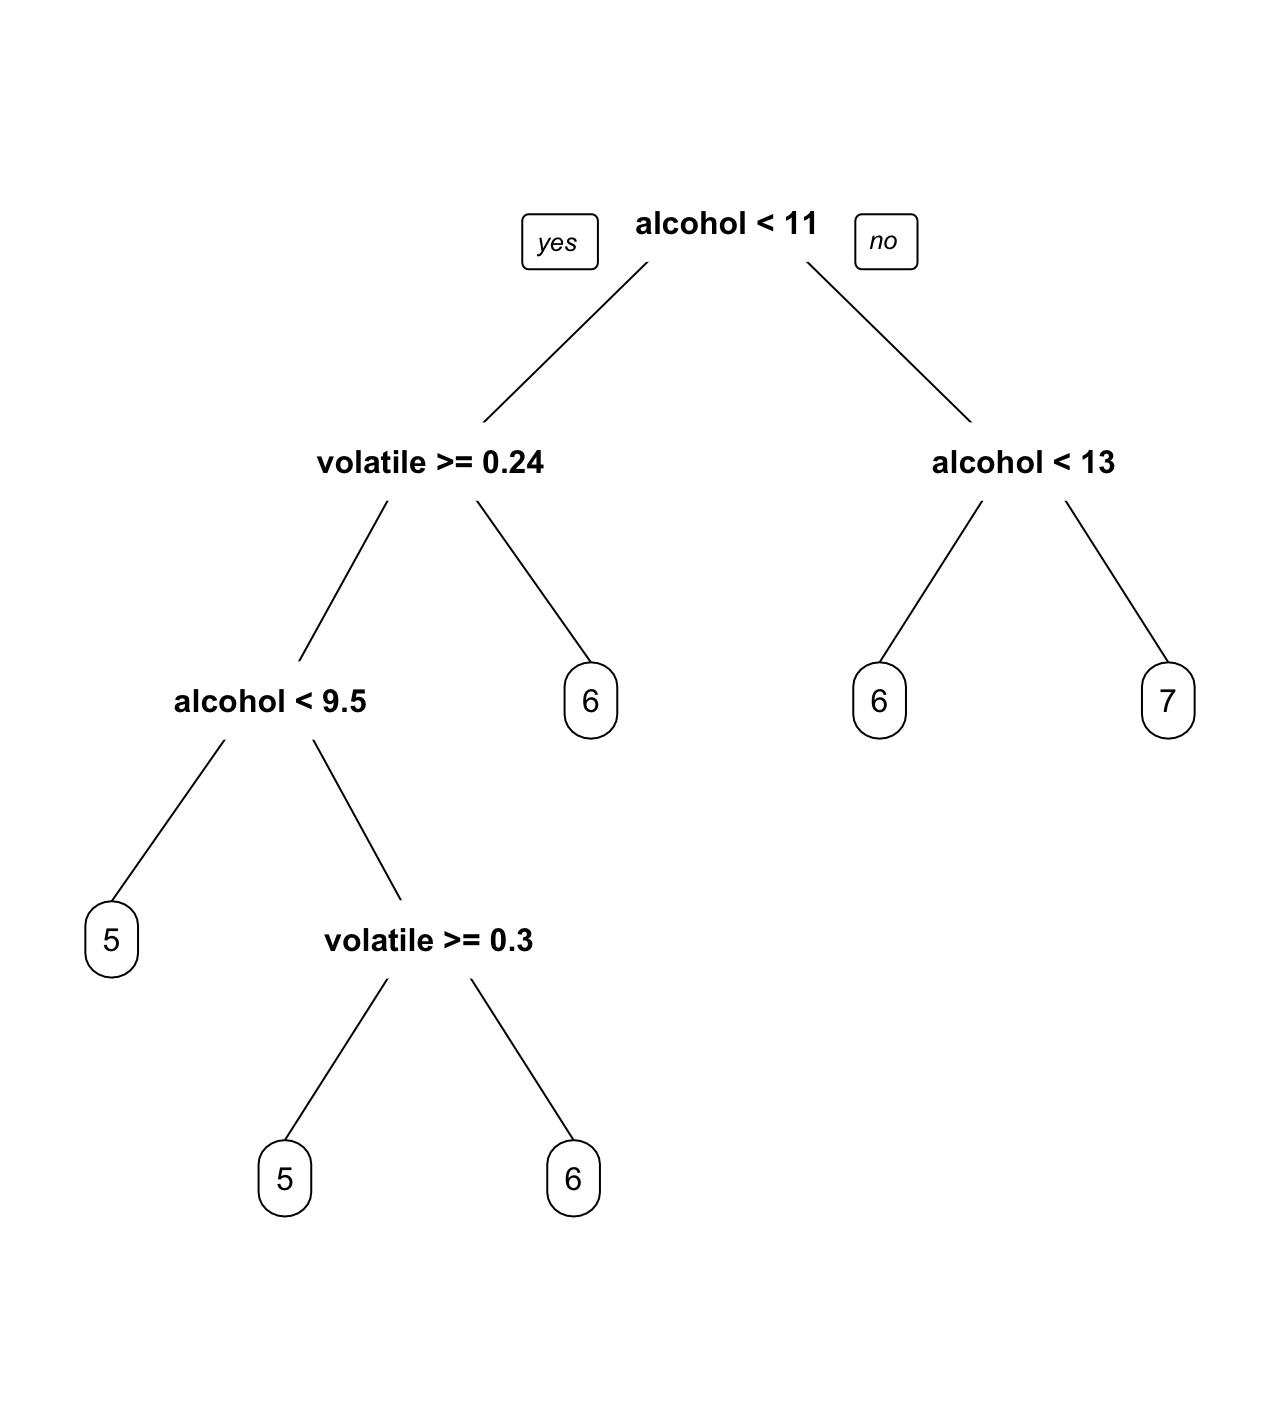
\includegraphics[width=160pt]{figure/Tree.png}
        				\end{center}
			\end{figure}
	\end{column}
	\begin{column}{0.5\textwidth}
			\begin{table}[htp]
							\resizebox{\textwidth}{!}{
					\begin{center}
						\begin{tabular}{c|ccccccc}
   & & & & tru & & & \\ 
prd  & 3  & 4 &  5 &  6 &  7 &  8 &  9\\ \hline
  3& 0& 0& 0& 0& 0& 0& 0 \\
  4& 0& 0& 0& 0& 0& 0& 0 \\
  5 &   1 &  11 & 82 & 44 &  4 &  0 &  0\\
  6  & 0  & 4  &58 &178&  64 & 11 &  1\\
  7  & 0  & 1  & 0  &10 & 16 &  5&   0 \\
  8 & 0 &0 &0 &0 &0& 0 &0 \\
  9 & 0 &0 &0 &0 &0 &0 &0 	
						\end{tabular}
					\end{center}
				}
			\end{table}		
	\end{column}
\end{columns}
}

\subsection{Random Forest}
\frame{
\frametitle{Random Forest}
\qquad $Error Rate = 0.3041$
\begin{columns}
	\begin{column}{0.5\textwidth}
				\begin{figure}
    				\begin{center}
        					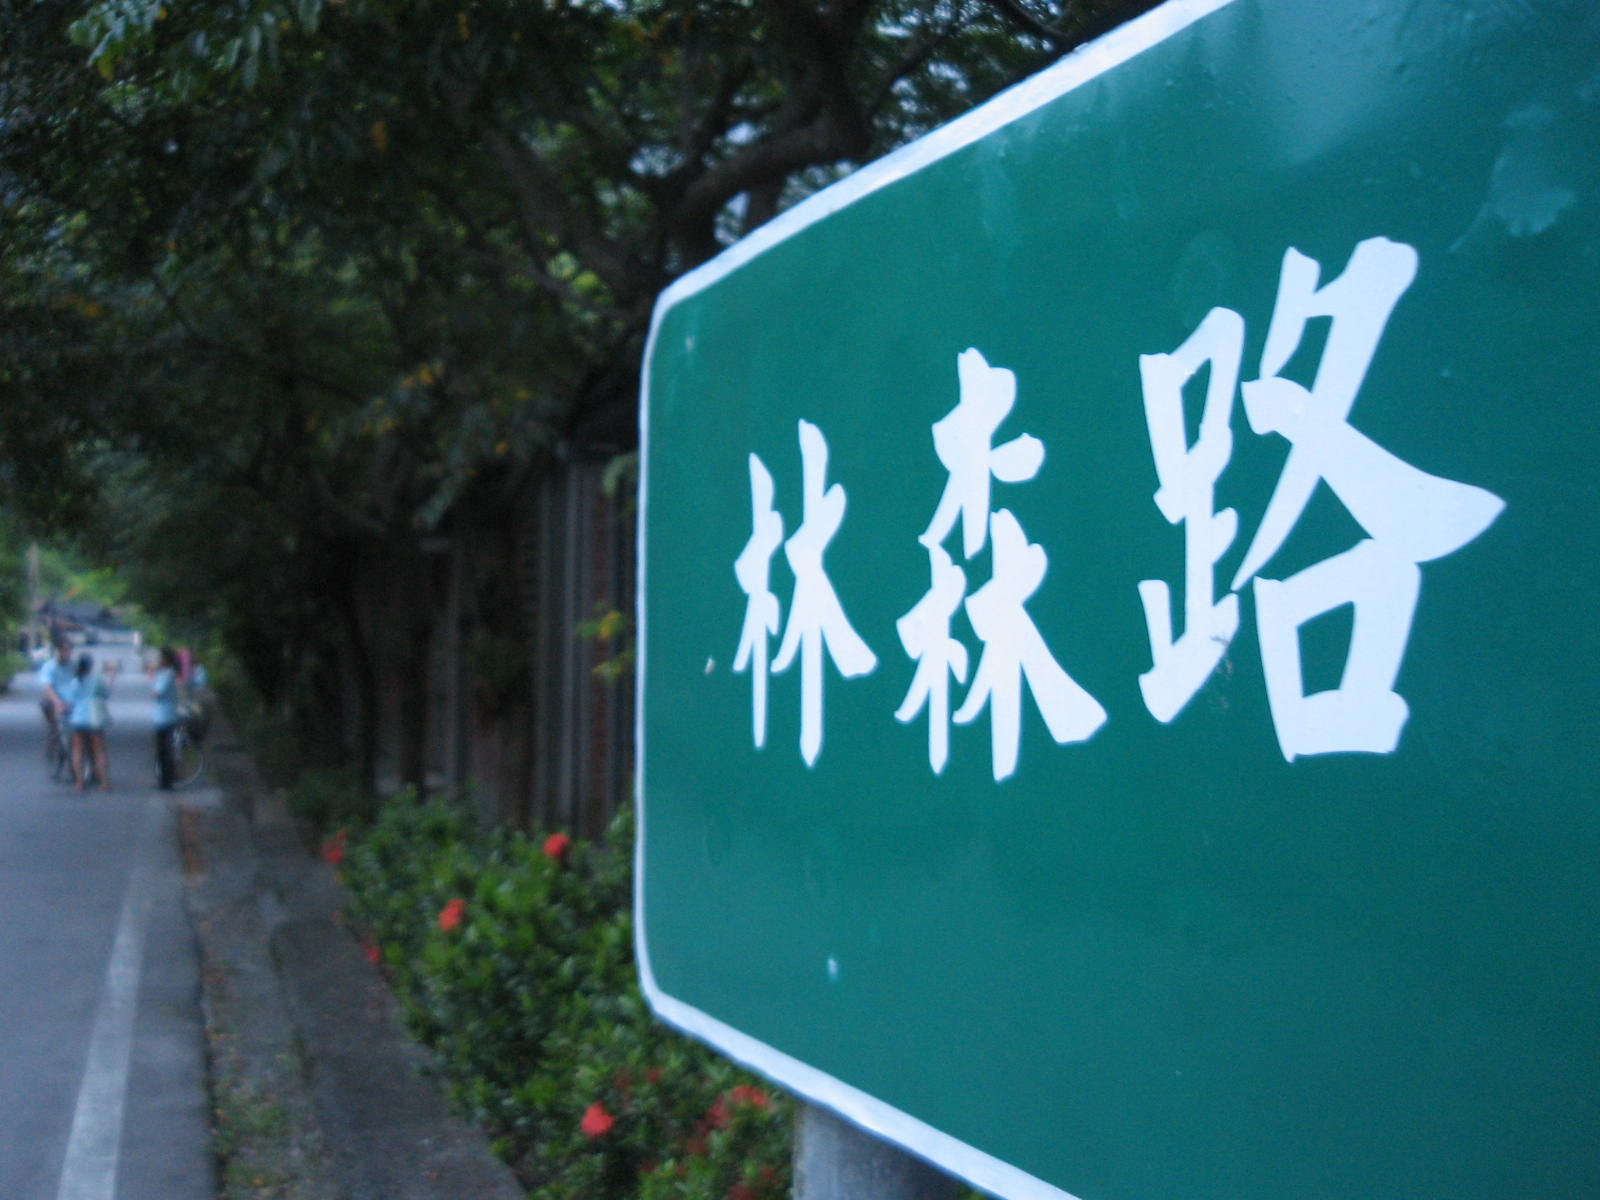
\includegraphics[width=160pt]{figure/RF.png}
        				\end{center}
			\end{figure}
	\end{column}
	\begin{column}{0.5\textwidth}
			\begin{table}[htp]
							\resizebox{\textwidth}{!}{
					\begin{center}
						\begin{tabular}{c|ccccccc}
   & & & & tru & & & \\ 
prd  & 3  & 4 &  5 &  6 &  7 &  8 &  9\\ \hline
  3& 0& 0& 0& 0& 0& 0& 0 \\
  4  & 0  & 3  & 1  & 0  & 0  & 0  & 0\\
  5  & 1  &10  &97 & 24  & 3  & 1 &  0\\
  6  & 0 &  3 & 42 &194 & 38 &  6 &  1\\
  7  & 0  & 0  & 0 & 14  &42  & 4  & 0\\
  8  & 0  & 0 &  0  & 0 &  1  & 5 &  0\\
  9 & 0 &0 &0 &0 &0 &0 &0 	
						\end{tabular}
					\end{center}
				}
			\end{table}		
	\end{column}
\end{columns}
}



\section{Conclusion}
\frame{
\frametitle{Conclusion}
\begin{columns}
	\begin{column}{0.3\textwidth}
		\begin{itemize}
		\item{The data is too unbalanced}
		\item{The random forest performs the best}
		\item{It is not bad while error rate = 0.5 }
		\end{itemize}
	\end{column}
	\begin{column}{0.7\textwidth}
				\begin{table}[htp]
					\begin{center}
						\begin{tabular}{c|rr}
                       &      MSE  &Error Rate\\ \hline
Full           &   0.7050 & 0.4650\\
Non-collinearity &0.7240   &0.4690\\
Final       &    0.7270  &0.4730\\
Best Subset     &      0.4970  & 0.4653\\
Lasso             &    0.5358 & 0.4776\\
PCR               &    0.5853&  0.5122\\
Decision Tree    &            NA &  0.4367\\
Random Forest   &             NA  & 0.3041
 						\end{tabular}
					\end{center}
			\end{table}		

	\end{column}
\end{columns}

}


\section{Reference}
 \frame{
\frametitle{Reference}
\begin{itemize}
	\item[1]{James, G., Witten, D., Hastie, T. and Tibshirani, R., \textit{An Introduction to Statistical Learning with Applications in R}, Springer, New York, 2013}
	\item[2]{Johnson, R. and Wichern, D. \textit{Applied Multivariate Statistical Analysis, 6th Edition}, Pearson, London, 2014}
	\item[3]{Kabacoff, R.I., \textit{R in Action Data, analysis and graphics with R}, Manning, New York, 2014}
	\item[4]{Matloff, N., \textit{The Art of R Programming, A Tour of Statistical Software Design}, No Starch Press, San Francisco, 2011}
	\item[5]{Montgomery, D.C., Peck, E.A. and Vining, G.G., \textit{Introduction to Linear Regression Analysis, 4 Edition}, Wiley, 2006}
\end{itemize}	
}

\end{document}
